\documentclass[conference]{IEEEtran}
\IEEEoverridecommandlockouts
% The preceding line is only needed to identify funding in the first footnote. If that is unneeded, please comment it out.
\usepackage{cite}
\usepackage{amsmath,amssymb,amsfonts}
\usepackage{algorithmic}
\usepackage{graphicx}
\usepackage{caption}
%\usepackage{subfigure}
\usepackage{subcaption}
\usepackage{mdframed}
\usepackage{mathtools}

\usepackage{textcomp}
\usepackage{listings}
\usepackage{multicol}
\usepackage{tikz}
\usepackage{multirow}
\usepackage{comment}
\usepackage{balance}

\newcommand{\fixme}[1]{{\color{red}\textbf{FIXME:} #1}}
\newcommand{\Ehsan}[1]{{\color{blue}\textbf{Ehsan:} #1}}
\newcommand{\Fatem}[1]{{\color{green}\textbf{Fatemeh:} #1}}
\newcommand{\Marjan}[1]{{\color{cyan}\textbf{Marjan:} #1}}

\usepackage{xcolor}
\def\BibTeX{{\rm B\kern-.05em{\sc i\kern-.025em b}\kern-.08em
		T\kern-.1667em\lower.7ex\hbox{E}\kern-.125emX}}
\newcommand{\conn}{\!\rightsquigarrow\!}
\newcommand{\nconn}{\!\mathrel{\hspace{.1em}\not\hspace{-.1em}\rightsquigarrow}\!}
\newcommand{\overto}[1]{\stackrel{#1}{%
		\overrightarrow{\smash{\,{\phantom{#1}}\,}}}}

%-------------------------
\lstdefinelanguage{rebeca}{
	morekeywords={reactiveclass, knownrebecs, statevars, main, msgsrv, constraints,con, main, define, LTL, CTL, boolean, int, shortint, byte, if, else, while, for, wait, msg, reset, set, self, false, true, now, after, delay, deadline, initial, unicast, succ, unsucc},
	otherkeywords={=>,<-,<\%,<:,>:,\#,@},
	sensitive=true,
	morecomment=[l]{//},
	morecomment=[n]{/*}{*/},
	morestring=[b]",
	morestring=[b]',
	morestring=[b]"""
}
%\captionsetup[lstlisting]{font={small}}
\lstset{
	language=rebeca,
	aboveskip=3mm,
	belowskip=3mm,
	showstringspaces=false,
	columns=flexible,
	xleftmargin=10mm,
	% basicstyle={\myttsize\ttfamily},
	basicstyle={\small},
	keywordstyle=\color{blue},
	numbers=left,
	numberstyle=\color{black},
	numbersep=7pt,
	stepnumber=1,
	breaklines=true,
	breakatwhitespace=true,
	tabsize=2,
	numberblanklines=false,
	frame=l
}

\begin{document}
	
	\title{%Reactive Actors in Isolation for Efficient Analysis \\
	Reactive Actors: Isolation for Efficient Analysis of Distributed Systems
		%\thanks{The authors would like to acknowledge DPAC and SEADA.}
	}
	
	\author{\IEEEauthorblockN{Marjan Sirjani}
\IEEEauthorblockA{
\textit{School of Innovation, Design and Engineering} \\
\textit{M{\"a}lardalen University}\\
V{\"a}ster{\aa}s, Sweden \\
\textit{School of Computer Science} \\
\textit{Reykjavik University}\\
Reykjavik, Iceland \\
marjan.sirjani@mdh.se}
		\and
		\IEEEauthorblockN{Ehsan Khamespanah}
\IEEEauthorblockA{\textit{School of Computer Science} \\
\textit{Reykjavik University}\\
Reykjavik, Iceland \\
\textit{ School of ECE} \\
			\textit{University of Tehran}\\
			Tehran, Iran \\
ehsank@ru.is}
		\and
		\IEEEauthorblockN{Fatemeh Ghassemi}
		\IEEEauthorblockA{\textit{ School of ECE} \\
			\textit{University of Tehran}\\
			Tehran, Iran \\
			fghassemi@ut.ac.ir}
	}
	
	\maketitle
	
	\begin{abstract}
	In this paper we explain how the isolation or decoupling of actors can help in developing efficient analysis techniques. The Reactive Object Language, Rebeca, and its timed extension are introduced as actor-based languages for modeling and analyzing distributed systems.
	%
%	and will explain our theories, techniques and tools for model checking and performance evaluation of such models.  Rebeca can be used to model asynchronous event-based components in systems, and in the extended version, Timed Rebeca, real time constraints can be captured in the language. We will explain how the isolation of actors, meaning no shared variable, non-preemptive execution of event handlers, and no blocking send or receive, help in developing more efficient analysis techniques. 
We show how floating-time transition system can be used for model checking of timed actor models when we are interested in event-based properties, and how it helps in state space reduction. We explain how the model of computation of actors helps in devising an efficient state distribution policy in distributed model checking. We show how we use Rebeca to  verify the routing algorithms of mobile adhoc networks. The paper is written in a way to make the ideas behind each technique clear such that it can be reused in similar domains.
		
		%I will show different applications of our approach including analysing a wireless sensor network application, mobile ad-hoc network protocols, network-on-chip designs, and a macroscopic agent-based simulation of urban planning.
	\end{abstract}
	
	\begin{IEEEkeywords}
		Actors, real-time  systems, distributed systems, model checking\end{IEEEkeywords}
	
%\fixme{Where should the acknowledgement be?}
\section{Introcution} \label{sec::introduction}

\Marjan{Add your comments in others' sections in color}
\Ehsan{blue}
\Fatem{green}

%Message of the paper: The actor-based language, Rebeca, provides a usable and analyzable model for distributed, concurrent, event-based asynchronous systems (Cyber-Physical systems).

%Distributed systems  are defined like this
%IBM: A distributed computer system consists of multiple software components that are on multiple computers, but run as a single system. The computers that are in a distributed system can be physically close together and connected by a local network, or they can be geographically distant and connected by a wide area network. ...distributed system contains multiple nodes that are physically separate but linked together using the network. All the nodes in this system communicate with each other and handle processes in tandem. Each of these nodes contains a small part of the distributed operating system software.

Distributed systems consist of software components executed on different computers that are linked together by a network. The software components communicate with each other in order to achieve the goal of the distributed system.
Nowadays distributed systems are everywhere providing scalability and redundancy.  Design and analysis of such systems is overly challenging.

%Reactive systems are defined like this
%Actor-based languages and distributed systems
Actor model is a model of concurrent computation for developing parallel, distributed and mobile systems \cite{Hewitt:77:Actors,Agha:97:ActorComputation}. Each actor is an autonomous object that operates concurrently, and  send and receive messages asynchronously.
%
Rebeca \cite{DBLP:journals/fuin/SirjaniMSB04,DBLP:conf/fmco/Sirjani06} is an actor-based language proposed to bridge the gap between software engineers and formal methods community.
Rebeca comes with a formal semantics and is the first actor-based language with model checking support \cite{DBLP:journals/csur/BoerSHHRDJSKFY17}.


Models can be used for both synthesis and analysis \cite{DBLP:conf/facs2/LeeS18}. We build abstract models that serve as a specification of a system to be built, and then we refine the models, adding
details until we build the system itself. The process is usually iterative, with
the specifications evolving along with their refinements. We may have different analysis purposes like verification, validation, and performance evaluation. 
Model checking, simulation, and building physical prototypes can all be used as methods for analysis. Simulation, which is the execution of an executable
model, reveals one possible behavior of a model with one set of inputs. Model
checking reveals all possible behaviors of a model over a family of inputs \cite{DBLP:conf/facs2/LeeS18}.
%If we have formal and automatic refinement techniques, we may be able to avoid introducing errors in the refined models while details are added. In this case, synthesis is said to be “correct by construction.”


%Why actors are good models for distributed systems?
%\noindent\textbf{Faithful models for distributed reactive systems} %\label{sec::Faithfulness}
%How models shape the thought and ease the analysis

%From Rocco paper: 
According to De Nicola et.al. in \cite{DBLP:conf/coordination/NicolaFPT18} a major challenge in designing languages is to devise appropriate abstractions and linguistic primitives to deal with the specificities of the domain under investigation.
%
%From Gul and Rajesh: 
%http://web.cs.ucla.edu/~palsberg/course/cs239/papers/karmani-agha.pdfA 
Karmani and Agha believe that a programming language should facilitate the process of writing programs by being close to the conceptual level at which a programmer thinks about a problem, rather than at the level at which it may be implemented \cite{DBLP:reference/parallel/KarmaniA11}. 

In \cite{DBLP:conf/birthday/FriendlinessSirjani18}, Sirjani defines faithfulness as the similarity of the
model and the system; and it is argued that faithfulness can bring in analizability and tracability. 
According to \cite{DBLP:conf/birthday/FriendlinessSirjani18}, a modeling
language is faithful to a system if the model of computation supported by the
language matches the model of computation of [the features of interest of] the
system. 
In \cite{Ptolemy:14:Book} a model of computation (MoC) is defined as a collection of rules that govern
the execution of the [concurrent] components and the communication between
components.
Faithfulness can be seen as the key motivation behind domain-specific
languages.


In the following section we explain what we mean by isolation of actors and how it can help in analysis. We then focus on a model that is presented as the semantics of Timed Rebeca and can help by a significant amount of reduction in the state space while doing the analysis. We believe that similar techniques can be used in different analysis methods for event-based reactive isolated modules. 
%
In Section \ref{sec::DMC}, we present a technique used for analysis by distributed model checking which is specific for actors and Rebeca.
%
Section \ref{sec::wrebeca} explains how we deployed special techniques to make analysis of  mobile adhoc networks possible.

%\noindent\textbf{Analysis of distributed systems and isolated actors.}
\section{Analysis of Distributed Systems and Isolated Actors}
For explaining our approach, we distinguish three levels of abstraction: the distributed software system itself with all the implementation details, the modeling language which is Rebeca here, and the generated state space which is built for the sake of analysis and  we model it as a state transition system. There are alternative ways for analysis, like using logical theorems and applying reasoning based on that, but here we use different variations of state transition systems.
We sometimes call the transition system the semantics of our model as it shows the behavior in a formal way.


Active objects and actors are encapsulated modules with no shared variables. In Rebeca, we also choose to have atomic execution of message servers (i.e. methods, or event handlers) which gives us a macro-step semantics and models a non-preemptive execution of the handlers.
Our actors are reactive, when sending a message they are not blocked and there is no explicit receive. So, there is no coupling via shared variables, no coupling because of waiting for another actor to return a value for a remote procedure call, and no coupling because of a context dependency caused by having a \textit{future}  construct in the language.
This isolation of actors helps in more efficient analysis, and reduces the state space.
Moreover, if we are only interested in the event-based properties we may be able to abstract even more and just keep the states that are followed by a transition which we are interested in. This type of reduction is not straight forward as we need to prove that we are preserving the order of the events while abstracting away some of the states and transitions. 
%This is what is done in partial order reduction.

Floating Time Transition System is a natural event-based semantics for timed actors, giving us a significant amount of reduction in the state space, using a non-trivial novel idea.
	
%paragraphs in the Intro
%%\section{Reactive Systems} \label{sec::reactive-systems}
\paragraph{Reactive Systems} \label{sec::reactive-systems}
%%\section{Reactive Actors} \label{sec::reactive-actors}
\paragraph{Reactive Actors} \label{sec::reactive-actors}
%\section{Faithful Models for Reactive Systems} \label{sec::Faithfulness}
From Rocco paper: a major challenge in designing languages is to devise appropriate abstractions and linguistic primitives to deal with the specificities of the domain under investigation.

\section{Timed Rebeca and Floating Time Transition System} \label{sec::FTTS}


\begin{figure}[!htbp]
 	\begin{center}
 		\small
 		\begin{mdframed}
 			\begin{align*}
 				\mathit{Model} &\Coloneqq  Class^* ~ Main \qquad \\
 				Main &\Coloneqq \mathbf{main} ~ \{ ~ InstanceDcl^* ~ \} \qquad \\
 				InstanceDcl &\Coloneqq \mathit{className} ~ \mathit{rebecName}~(\langle rebecName \rangle ^*) \\
 							& ~~~ : (\langle literal \rangle ^*);\\
 				Class &\Coloneqq \mathbf{reactiveclass} ~ className ~ \{ \\
 					  &\ ~~~ ~ \mathit{KnownRebecs} ~ \mathit{Vars} ~ \mathit{MsgSrv}^* ~ \}\\
 				KnownRebecs &\Coloneqq \mathbf{knownrebecs} ~ \{ ~ \mathit{VarDcl}^* ~ \} ~ \\
 				\mathit{Vars} &\Coloneqq \mathbf{statevars} ~ \{ ~ \mathit{VarDcl}^* ~ \} ~ \\
 				\mathit{VarDcl} &\Coloneqq type ~ \langle v \rangle ^+;\\
 				MsgSrv &\Coloneqq \mathbf{msgsrv} ~ methodName(\langle type ~ v \rangle ^*) ~\\
				             &\ ~~~  \{ ~ Stmt^* ~ \} \\
 				Stmt &\Coloneqq v = e; ~| ~ v = ?(e\langle ,e \rangle^+); ~| ~ Call;| ~ \\
 					 &\ ~~~  ~ {\it if} ~ (e) ~ \{ ~ Stmt^* ~ \} ~ [else ~ \{ ~ Stmt^* ~ \}]; |   \\
					 &\ ~~~ ~ \mathbf{delay}(t); \\
 				Call &\Coloneqq rebecName.methodName(\langle e \rangle ^*) \\
 					 &\ ~~~  [\mathbf{after}(t)]  [\mathbf{deadline}(t)]\\
			%\\
			%	& \text{(a) Abstract Syntax of Rebeca}
 			\end{align*}
 		\end{mdframed}
 		\caption{Abstract syntax of Timed Rebeca (from \cite{DBLP:journals/scp/KhamespanahSSKI15}). Angled brackets $\langle$...$\rangle$ are used as meta parenthesis, superscript $+$ for repetition at least once, superscript $*$ for repetition zero or more times, whereas using $\langle$...$\rangle$ with repetition denotes a comma separated list. Brackets $[...]$ indicates that the text within the brackets is optional. Identifiers $className$, $rebecName$, $methodName$, $v$, $literal$, and $type$ denote class name, rebec name, method name, variable, literal, and type, respectively; and $e$ denotes an (arithmetic, boolean or nondetermistic choice) expression.
 		\fixme{Add the part about queue length and parameters to the constructor - Check that the syntax is consistent in the three model that we have}}
 		\label{fig::TRebecaSyntax}
 	\end{center}
 \end{figure}


Floating Time Transition System (FTTS) is proposed based on the isolation of timed rebecs \cite{DBLP:conf/facs2/KhamespanahSVK15,DBLP:journals/scp/KhamespanahSSKI15}. The idea behind FTTS is similar to partial order reduction (POR) but the technique does not fit exactly in the definition of POR. 
%
In POR we exploit the commutativity of concurrently executed transitions, which result in the same state when executed in different orders. So, we can only expand a representative subset of all enabled transitions and abstract the rest away while preserving the properties of interest. %This way the properties are preserved. 
%
If we consider the standard Timed Transitions System semantics (TTS) of Timed Rebeca, we cannot say that FTTS is derived from TTS by POR, because we are not only abstracting away some of the transitions we are also changing the states. You cannot necessarily find one state in FTTS which is the same as a state in TTS. Both states and transitions are changed while the order of events are preserved (you may see the proof of property preservation in \cite{DBLP:conf/facs2/KhamespanahSVK15}).
%

What we mean by floating time is that in each state of the state space, different actors do not necessarily have the same local clock, i.e.,  actors are not synchronised on their local time in the state space. We consider this as letting the time \textit{float} across the actors in the state space. 
To avoid confusion, it is important to note the different models in different levels of abstraction, and also layering of models. We have (1) distributed systems, we use (2) Timed Rebeca to model distributed systems, and we model (3) the state space as Floating Time Transition System to do the analysis. 
%
Note that at the level of Timed Rebeca, actors have synchronised local clocks which gives us a notion of global time across the model. We use time stamps, and time stamps are comparable across all actors in the model. This makes our model simpler and more understandable, and our analysis more efficient.
But in distributed systems we cannot assume synchronised clocks and time stamps for distributed software components, at least not for free \footnote{Ptides\cite{DBLP:conf/dsrt/DerlerLM08} and Spanner\cite{Corbett:2013:SGG:2518037.2491245} are two examples that assume synchronized clocks  (up to an error bound) and use logical time stamps.
They proposed certain mechanisms to be able to have such assumption.}. 
For that assumption to be valid and faithful enough to the system,  we rely on the layering and different responsibilities for different layers. For distributed actors (as faithful representatives of distributed software components) to be able to have synchronised clocks and comparable time stamps we rely on the lower-level network protocols to provide that for us. 

In Timed Rebeca we have a concept of time and we can consider that each statement is executed at a certain point in time. Note that we are now talking at the level of the Rebeca model, the notion of time is the model time, and we do not need to worry about synchronising the clocks among different components in the distributed system (which are modeled as actors in our Rebeca model). We assume that local clocks of actors are synchronised and we  have time stamps on each statement  in the actors which are comparable across the actors.

In Timed Rebeca models, we use a \texttt{delay(t)} statement to show the computation delay. Other statements are assumed to be executed in zero time. We use  \texttt{after(t)} in combination with a \texttt{send} message statement, it means that the time stamp of the message when it is put in the queue of the receiver is the value of the local clock of the sender (\texttt{now} in the sender) plus the value of \texttt{t}.
The progress of time is forced by the \texttt{delay} statement and also by \texttt{after}. 
We can assume that the time stamp of all the statements are zero when a model starts to execute, then in each actor the local time is increased by value of \texttt{t} if there is a \texttt{delay(t)} statement.
A \texttt{send} statement with an  \texttt{after} does not cause any increase in the local time per se. The statement following the \texttt{send} statement has the same time stamp as the \texttt{send} statement itself.
The \texttt{after} construct may cause an increase in the time when the actor picks the message annotated by \texttt{after} to be executed. The local time of the receiver actor is set to the time stamp of the message, unless it is already greater than that.
The latter situation means that the message  sits in the queue while the actor is busy executing another message.
Remember that messages are executed atomically and are not preempted.
%
The progress of time happens in the case that the time stamp of the message is greater than the local time of the receiver actor, the local time will be pushed forward.
%
The \texttt{after} construct can be used to model the network delay, and also to model periodic events.


If we use the standard Timed Transition System (TTS) to generate the state space for Timed Rebeca model we distinguish three types of transitions: $\tau$ transitions, \textit{events}, and \textit{timed} transitions.
In FTTS we reduce that to only \textit{events} transitions.
%
We explain TTS and FTTS for Timed Rebeca using an example in Listing \ref{src::FTTS-actor-model}.
Listing \ref{src::FTTS-actor-model} shows a simple Rebeca model with two rebecs $r1$ and $r2$ instantiated from two reactive classes $RC1$ and $RC2$.
$RC1$ has only one message server ($m1$) in which it triggers the two message servers of $RC2$ ($m2$ and $m3$).
The two message servers of $RC2$ are event handlers that do nothing, i.e., there are no internal actions caused by statements like assignments, or \texttt{send}, and no  \texttt{delay} statements. Note that \texttt{send} statements are considered as internal or silent actions but they cause a change in the message queue of the receiver by adding the sent message to that queue.
 

Figure \ref{fig::FTTSandTTS}.a shows the TTS generated for the model in Listing \ref{src::FTTS-actor-model}. 
The constructor of $RC1$ puts the message $m1$ in the queue of $RC1$. So, in $time=0$ we have the message $m1$ in the queue of $r1$ (see state $s_0$ in Figure \ref{fig::FTTSandTTS}.a). Also, you see that the message queue of $r2$ is empty. On the transition from $s_0$ to $s–1$ the message is taken from the queue of $r–1$, and in the state $s_1$ the method $m_1$ is ready to be executed, i.e., the Program Counter (PC) is at $m1:1$. The first statement in $m_1$ is a \texttt{delay} statement which is executed and pushes the time forward to $time=2$ in state $s_2$.
In the state $s_2$, the PC points at a $send$ statement: $r_2.m_2()$. After this statement is executed as a silent or $\tau$ statement, we move to the state $s_3$ and have the message $m_2$ in the queue of $r–2$. The message $m_2$ is shown as $(m_2(), 2, \infty)$ in which $2$ is the timestamp of the message and $\infty$ is the value of \texttt{deadline}. The message can only be taken if and when the current time of receiver is greater than or equal its timestamp. If the current time of receiver is less than the timestamp and there is no transition of types  $\tau$  or \textit{event} enabled then the time of the receiver is advanced to the value of the timestamp (transition of type \textit{time}) and only then the message can be taken.


On the transition from $s_3$ to $s_4$ the message $m_2$ is fetched to be executed, but the body of the message server $m_2$ is empty so nothing happens. We move from $s_4$ to $s_5$ by executing another \texttt{delay} statement and the time is progressed to four.
At state $s_5$ the \texttt{send} statement is executed, the message is put in the queue of $r_2$ and we will get to the state $s_6$.
At state $s_6$, two transitions are enabled and each can be  executed first non-deterministically. 
We go to the state $s_7$ if the message in the queue of $r_2$ is taken and executed first. We go to the state $s_8$ if the \texttt{send} statement at $m_1:5$  is executed first and then the message $m_1$ is put in the queue of $r_1$. No matter which trace in the diamond shown in the Figure \ref{fig::FTTSandTTS}.a is taken, we will get to the state $s_9$.
In the state $s_8$, although there is one message in the queue of each rebec, only one transition is enabled. The reason is that   the message in the queue of $r_1$ has the timestamp of $14$ (because of the \texttt{after(10)} attached to the \texttt{send} statement).
Only in the state $s_9$, when there are no transitions of types $\tau$ or \textit{event}  enabled the transition of type \textit{time} is taken, and time is advanced for $10$ units of time. Now, at the state $s_{10}$ finally the message $(m_1(), 14,\infty )$ is enabled.

The FTTS for Listing \ref{src::FTTS-actor-model} is shown in Figure \ref{fig::FTTSandTTS}.b. From this figure you may observe that the only transitions in FTTS are the transitions of type \textit{event}, and you may also notice the reduction in the state space.
%
The relation between TTS and FTTS of a Timed Rebeca model is not trivial and cannot be explained as partial order reduction, i.e., you may find states in FTTS which are not in TTS.
For example in Figure \ref{fig::FTTSandTTS} for $3$ out of $5$ states in FTTS there are no similar states in TTS. Nevertheless, in \cite{DBLP:conf/facs2/KhamespanahSVK15} we proved a bisimulation relation between FTTS and TTS to prove that the order of events is preserved in FTTS.

 It is not easy to understand the FTTS semantics of Timed Rebeca if we start from the standard TTS semantics. A better way is to start from the Timed Rebeca model, and think of an event-based semantics. By focusing on the event-based properties as the properties of interest, we narrow down the interesting transitions to the \textit{event} transitions which are taking the messages from the queue and executing the corresponding message server.
This way, we have macro-step semantics where on each transition we take the enabled event (i.e. message) and execute the corresponding message server all in one transition. This is similar to the original semantics of Rebeca presented in \cite{DBLP:journals/fuin/SirjaniMSB04}, but here we have messages in the queue tagged by timestamps (in Timed Rebeca we usually call the message queues the message bag with time-tagged messages). The main technical point here is how to choose the message to take next. The algorithm for making the state space looks into the queues of all the rebecs and picks the message that is enabled \textit{earlier} than the others.  The tricky point is to get the definition of \textit{enabled earlier} correctly. The first idea that comes to mind is to pick the message with the least timestamp, but we also need to check the current time or \textit{now} of the receiver rebec. If the value of \textit{now} is larger than the timestamp then that would be the time that the message can really be taken. So,  for each rebec we need to find the maximum between  the timestamps and the value of  \textit{now} of the receiver rebec, and we need to do that for all the rebecs and all the messages in their queues,  and find the least among these values. That would be the message that will be taken first and will be the event on the next transition. There may be more than one message with that characteristic, and in that case the choice is nondeterministic.


\Marjan{I should add about BFTTS}

\begin{lstlisting}[language=rebeca, caption= A simple Timed Rebeca model with two rebecs, label=src::FTTS-actor-model]
reactiveclass RC1 (3) {
	knownrebecs {
		RC2 r2;
	}
	RC1() {
		self.m1();
	}
	msgsrv m1() {
		delay(2); %PC = 1
		r2.m2();  %PC = 2 
		delay(2); %PC = 3 
		r2.m3();  %PC = 4
		self.m1() after (10); %PC = 5
	}
}
reactiveclass RC2 (4) {
	knownrebecs {
		RC1 r1;
	}
	RC2() { }
	msgsrv m2() { }
	
	msgsrv m3() { }
}

main {
	RC1 r1(r2):();
	RC2 r2(r1):();
}

\end{lstlisting}

\begin{figure}
\centering
\begin{subfigure}[b]{0.34\textwidth}
%\subfigure[TTS]{
%\label{fig::TTS}
  \centering
  \small{
   \includegraphics[width=.8\textwidth]{resources/TTS.pdf}
  }
  \caption{TTS}
  \label{fig::TTS}
%}
\end{subfigure}
%\qquad
\begin{subfigure}[b]{0.14\textwidth}
%\subfigure[FTTS]{
%\label{fig::FTTS}
  \centering
  \small{
   \includegraphics[width=.8\textwidth]{resources/FTTS.pdf}
   \caption{FTTS}
   \label{fig::FTTS}
  }
%}
\end{subfigure}
\caption{ TTS and FTTS for the Timed Rebeca model in Listing
\ref{src::FTTS-actor-model}.
\fixme{Shall we add one more state to TTS such that the end transitions are the same?}}
\label{fig::FTTSandTTS}
\end{figure}

\begin{figure}
\centering
\includegraphics[width=.15\textwidth]{resources/BFTTS.pdf}
\caption{ Bounded FTTS for the Timed Rebeca model in Listing \ref{src::FTTS-actor-model}.}
\label{fig::BFTTS}
\end{figure}

\section{Distributed Model Checking} \label{sec::DMC}
In addition to benefiting from the isolation of actors for reducing the size of state spaces, this property can be used for more efficient analysis of huge state spaces. A major limiting factor in applying model checking for the analysis of real-world systems is the huge amount of space and time required to store and explore state spaces. Distributed model checking is a technique for analyzing these types of state spaces; in which, state spaces are partitioned into some slices and each slice is assigned to a computational node to be analyzed. The efficiency of this technique depends on the communication costs among computational nodes which is related to the distribution policy of states among nodes \cite{DBLP:journals/entcs/OrzanPE05}. Another, more fine-grained, representative of communication cost is the number of split transitions; a split transition is a transition between two states,  where the hosts of source and destination states are different nodes. In \cite{DBLP:journals/eceasst/KhamespanahSMSR15} we showed how the actor model can be used to reduce teh number of split transitions. We introduced a new state distribution policy based on the so-called Call Dependency Graph (CDG) of actor models. A CDG represents the abstract causality relation among messages of actors. Our abstraction is akin to the dynamic representation of actor's event activation causality proposed by Clinger \cite{clinger}. 

The most primitive and widely used distribution policy is random state distribution \cite{DBLP:journals/entcs/GaravelMS13}. Random state distribution policy distributes states among nodes based on their hash values. Random distribution policy guarantees load balancing. However, it is not an effective technique as cycles are scattered over many different nodes. In \cite{DBLP:journals/entcs/OrzanPE05}, another state space distribution policy is suggested to improve the locality of cycles. This policy is based on the static analysis of an abstracted model and detects \emph{may} or \emph{must} transition relations among states \cite{DBLP:conf/lics/LarsenT88}. Based on this analysis, if two states have a \emph{must} relation, they should be stored in a same node. We use a similar idea in our state distribution policy and show that using the CDG improves the locality of cycles by reducing the split transitions in the state space. In other words, we find the \emph{must} relations among the states of actor models using the CDG. Our technique is applicable to other service-oriented models where the unit of concurrency can be modeled as isolated autonomous active objects and message passing is the only way of communication. 

Clinger's event diagram comprise vertices (called \emph{dots}) for each event, and edges (called \emph{arrows}) that represent the activation relation of two events. Clinger's event diagram is typically drawn using parallel vertical swim-lanes for actors, where the dots are placed respecting their sequential execution order. Figure~\ref{fig::clinger} presents the Clingers' event diagram of an example actor model, shown in Listing~\ref{src::actor-model}. 

\begin{lstlisting}[language=rebeca, caption=An example of a simple actor model, label=src::actor-model]
reactiveclass AC1 {
  knownrebecs {AC2 ac2;}
  AC1() {
    self.msg1();
  }
  msgsrv msg1() {
    self.msg2();
    ac2.msg3();
  }
  msgsrv msg2() {
    self.msg1();
    ac2.msg4();
  }
}
reactiveclass AC2 {
  knownrebecs{AC1 ac1;}
  statevars{int sv;}
  AC2() {
    sv = 1;
  }
  msgsrv msg3() {
    ac1.msg1();
  }
  msgsrv msg4() {
    if (sv == 1)
      sv = 4;
    else
      sv = 3;
  }
}
main {
    AC1 ac1(ac2):();
    AC2 ac2(ac1):();
}
\end{lstlisting}

Clinger's event diagrams can be seen as the detailed representations of CDG. Intuitively, a CDG represents the possible activation relations of events derived from a static analysis of the model. Note that as actors are isolated, the only mechanism which may results in activating an event (causality among events) in an actor is sending a message to it. This way, the activation relation of events in a CDG can be extracted from the source codes of actor models by figuring out the message passing among actors. Using static analysis to find message passing results in over-approximatation of events activations in CDGs. Figure \ref{fig::cdg} illustrates the CDG which corresponds to the Clinder's event diagram of Figure \ref{fig::clinger}.

\begin{figure}
\centering
\subfigure[Clinger event diagram of an example actor model]{
\label{fig::clinger}
  \centering
  \small{
   \includegraphics[width=.18\textwidth]{resources/clinger.pdf}
  }
}
\qquad
\subfigure[CDG of an example actor model]{
\label{fig::cdg}
  \centering
  \small{
   \includegraphics[width=.18\textwidth]{resources/cdg.pdf}
  }
}
\caption{Clinger event diagram versus CDG of an example actor model.}
\label{fig::clinger-cdg}
\end{figure}

In \cite{DBLP:journals/eceasst/KhamespanahSMSR15} we designated and proved a relation between the cycles in the CDG and the cycles in state spaces. We devised a distribution policy for the distributed model checker of \emph{Rebeca} based on the CDG. The new distribution policy increases the efficiency of distributed model checking by increasing the locality of the accepting cycles. Experimental evidence supports that this new policy improves cycle locality, and decreases model checking time and memory in practice.
\section{Verification of Mobile Ad-hoc Protocols}\label{sec::wrebeca} 
%The computational model of Timed Rebeca makes it a faithful framework for modeling and analyzing network protocols based on asynchronous message passing, e.g., wireless protocols exploited in decentralized wireless networks.  
In decentralized wireless networks there is no pre-existing infrastructure, such as routers in wired networks or access points in managed (infrastructure) wireless networks, so nodes continuously send messages to each other to self-configure the network on ad hoc. %Wireless Ad-hoc protocols are mainly defined in terms of how each message type is handled, which accurately map with the concept of message handlers in Timed Rebeca. %As specifications of protocols, like IETF documents, are given in plain English, there are many ambiguities in their descriptions. So there are various implementations (with different behaviors and hence, behavioral properties) by different communities based on their impressions. The formal specification language of Timed Rebeca makes it an appropriate candidate to document such protocols for precise specification, clear comprehension, and analysis. We found many ambiguities in Ad hoc On Demand Distance Vector (AODV) [], a prominent routing protocol for Ad hoc wireless networks. We communicated with the IETF group to resolve the problems, documented the three last revision of AODV in []. 
Mobile Ad-hoc wireless networks (MANETs) consist of mobile nodes that freely move, so the underlying topology is dynamic. As wireless communication depends on the locality of nodes, i.e., the underlying topology, the behavior of nodes depends on the topology. Therefore, the correctness properties of MANETs are topology-dependent and hence, weaker in comparison with wired networks. For instance, one of the main properties of routing protocols is \emph{loop-freedom}, i.e., no established route stored in the routing tables visits the same node more than once. However, in MANETs, this property should hold for any mobility scenario. Another property for routing protocols is \emph{packet delivery}: always packets can be sent from a source to a connected destination. For MANETs, the packet delivery property is considered as whenever there is a path from a source to a destination for enough long period, any packet sent from a source can be received by the destination \cite{GlabbeekAWN}. Rebeca was extended in \cite{FOAC}, called wRebeca, to verify the topology-dependent properties of MANET protocols. To support modeling such protocols, wRebeca provides unicast, multicast, and broadcast for communication. %Thanks to its efficient analysis, we proposed an efficient version of AODV, precisely specified by wRebeca []. 
For instance, consider the specification of a node implementing Ad-hoc On Demand Vector (AODV) routing protocol \cite{AODV} in Figure \ref{code:aodv}. In this protocol when a node has data to send to a destination (${\it dip\_}$), informed by receiving ${\it rec\_newpkt}$ from the upper-layer application, it will initiate the \emph{route discovery} procedure if it has no routing to the destination in its routing table (${\it rst}[{\it dip\_}]$) by broadcasting a \emph{request} message (${\it rec\_rreq}$) at line $16$. Nodes upon receiving a request message, forward the request if they do not have any route to the destination until it reaches to the destination (line $24$). Now the destination replies by unicasting a \emph{reply} message (${\it rec\_rep}$) in response (line $26$) to the sender of the request (${\it oip\_}$). The reply message is regulated by the middle nodes until it arrives to the originator (line $48$).

\begin{figure*}
	\begin{center}
	%	\begin{lstlisting}[language=rebeca,multicols=2]
		\input{AODV.txt}
	%	\end{lstlisting}
	\end{center}
	\caption{The AODV protocol specified by wRebeca \label{code:aodv}\cite{FOAC}}
\end{figure*} 

The global states of a semantic model are defined by the local state of rebecs and the underlying topology. As mobility is the intrinsic characteristic of nodes, the dynamism of the topology is not explicitly defined as part of the protocol specification. Conversely, for each global state, there are a set of semantic transitions by which the underlying topology is implicitly changed.  For a network of $n$ nodes, there are $(n^2-n)/2$ possible links among them and by assuming the links are symmetrical, the state pace grows with a factor of $2^{(n^2-n)/2}$. To efficiently generate the semantic model of wRebeca, %as rebecs moves independently, 
we eliminate the topology from the global states and instead %define out of the have no shared variable, the semantic model can be  
%In the semantics of wRebeca, 
each semantic transition corresponds to the processing of an event as before while it is restricted to the set of topologies for which that behavior is valid.  We explain this by an example. Recall that a destination node upon receiving a request message unicasts a \emph{reply} message (${\it rec\_rep}$) to the node that has a route (called \emph{next hop}) to the sender $({\it oip\_})$ of the request (line $26$ in Figure \ref{code:aodv}). In the efficient semantic model for processing the ${\it rec\_rep}$ event, only two next states are considered; one for topologies in which the destination is connected to the next hop, and one for those that they are disconnected. These topologies are expressed in terms of \emph{network constraints} \cite{FatemehFI10,FatemehFI19}. Network constraints are a set of (dis-)connectivity relations between two addresses. For instance, ${\it and}({\it con}(n1,n2),!{\it con}(n3,n4)$ denotes that the nodes with addresses $n1$ and $n2$ are connected while $n_3$ and $n4$ are disconnected. To enforce a set of stable connectivity relations among the nodes, they can be specified in \emph{constraints} block at line $68$ of Figure \ref{code:aodv}. This approach reduces the state space substantially for real-world protocols and hence, makes the model checking technique possible as shown in Table \ref{Tab:aodv-redu}. When the number of nodes increases from $4$ to $5$, and the initial network constraint results $16$ possible topologies, the classic state space cannot be generated due to the memory limitation on a computer with 8GBRAM. The network constrains on transition are used during the model checking algorithm of \cite{FORM} or property specifications \cite{CSI2018} to verify the topology-dependent properties. 

\begin{table*}
	%   \renewcommand{\arraystretch}{1.5}
	\centering
	\caption{Comparing the size of state spaces with/without applying reduction \cite{FOAC}}
	\begin{tabular*}{0.75\textwidth}{@{\extracolsep{\fill }} |   c  c  r  r  r  r  |   }
		\hline
		  No. of & No. of valid & No. of states    &  No. of transitions     & No. of states & No. of transitions
		\\
		  nodes & topologies & before reduction  &  before reduction   & after reduction &  after reduction
		\\
		\hline	     
		 4 & 4 & 3,007 & 16,380 & 763  & 1,969 \\
		 4  & 8 & 12,327 & 113,480 & 1,554  & 3,804 \\
		 4  & 16 & 35,695 & 610,816 & 2,245 & 5,549 \\    
		 4  & 32 & 93,679 & 3,097,792 & 2,942 & 7,596 \\  
		 4    & 64  & 258,447  & 16,797,536 & 4,053 & 10,629 \\
		 5 & 16 & $>$655,441 & $>$11,276,879 & 165,959 &  598,342 \\
		\hline
	\end{tabular*}
	\label{Tab:aodv-redu}
\end{table*}

The reduction technique can be improved further if the topology be stable. As rebecs have no shared variable, the state space of network consisted of homogeneous nodes can be reduced by the \emph{counter abstraction} technique \cite{emerson1999asymmetry}. By this technique, the global state is defined by a vector of counters, one for each local state of nodes. If there are $n$ nodes in a network where each node can have $m$ possible local states, the global state is shown as $\langle c_1,\ldots,c_m \rangle $, where $c_i\le n$ denotes the number of nodes residing in the local state $i\le m$. Therefore, the state space is reduced from $m^n$ to $\begin{pmatrix}
n+m-1 \\
m \\
\end{pmatrix}$. To apply
counter abstraction concerning the topology, rebecs with an identical local state and
neighbors that are \textit{topologically equivalent} are counted together. Intuitively, all topologically equivalent nodes should be either all connected to each other, or disconnected, while they should have the same neighbors (except themselves). So if either one broadcasts, the same set of nodes (except themselves) will receive, and if they are also connected to each other, their counterpart (that is symmetric to the sender) will receive. For example, nodes $1,3$ and $2,4$ are topologically equivalent in Figure \ref{fig:topequiv}. To compute the reduced state space, nodes of the underlying topology are partitioned into the maximal sets of topologically equivalent nodes, and then a counter is considered for each pair of topology equivalence class and a local state that a rebec can be reside in. %, denoted by $\mathcal{N}_1,\ldots,\mathcal{N}_\ell$. We define the set of \textit{distinct local states} as $S^d=\bigcup_{c\in C}S_c$, and the set of topology equivalence classes as $\mathbb{T}=\{\mathcal{N}_1,\ldots,\mathcal{N}_\ell\} $.
% Consequently, each global state $( s_1,\ldots,s_n,\gamma)$ is
%abstracted into a vector of elements $(s^d_i,\mathcal{N}_i):c_i$ where $s^d_i\in S^d$, $\mathcal{N}_i\in\mathbb{T}$, and $c_i$ is the number of nodes in the topology equivalence class $\mathcal{N}_i$ that reside in the very local state $s^d_i$. Counting abstraction is beneficial when the reactive classes do not have a variable that will be assigned uniquely to its instances, such as  ``unique address" as a state variable. (Note that at the semantics, rebecs have identifiers which are not a part of their local states.)

 \begin{figure*}
 	\centering
 	\begin{subfigure}[b]{0.3\textwidth}
 		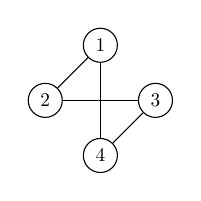
\begin{tikzpicture}[scale=.7, transform shape]
 		\node[style=circle,draw] (n1) at (1,2) {$1$};
 		\node[style=circle,draw] (n2) at (0,1) {$2$};
 		\node[style=circle,draw] (n3) at (2,1) {$3$};
 		\node[style=circle,draw] (n4) at (1,0) {$4$};
 		\draw (n1) edge (n2);
 		\draw (n1) edge (n4);
 		\draw (n3) edge (n2);
 		\draw (n3) edge (n4);
 		\end{tikzpicture}
 		\caption{A topology}
 		\label{fig:topequiv}
 	\end{subfigure}
    \begin{subfigure}[b]{0.6\textwidth}
    	\begin{tikzpicture}[scale=.8, transform shape]
    	\node [draw,outer sep=0,inner sep=3,minimum size=10] (n1) at (1,11) {$\begin{array}{l} 
    		1:(\{i\mapsto 1\},\epsilon),\\ 
    		2:(\{i\mapsto 2\},\langle{\it msg}\rangle),\\
    		3:(\{i\mapsto 1\},\epsilon),\\
    		4:(\{i\mapsto 0\},\epsilon),\end{array} %\begin{pmatrix}
    		%1 & 1 & 0 & 1 \\
    		%1& 1& 1 & 0 \\
    		%0 & 1  & 1 & 1 \\
    		%1 & 0 & 1 & 1
    		%\end{pmatrix}
    		$};
%    	\end{tikzpicture}
%    	\caption{Before applying counter abstraction}
%    	\label{fig::global}
%    \end{subfigure}
%    \begin{subfigure}[b]{0.3\textwidth}
%    	\begin{tikzpicture}[scale=.8, transform shape]
    	\node [draw,outer sep=0,inner sep=3,minimum size=10] (n2) at (7,11)
    	{$\begin{array}{l} ((\{i\mapsto 1\},\epsilon),\{1,3\}):\{1,3\},
    		\\((\{i\mapsto 2\},\langle{\it msg}\rangle),\{2,4\}):\{2\},\\
    		((\{i\mapsto 0\},\epsilon),\{2,4\}):\{4\}\end{array} $};
    	\draw[->, style=dashed] (n1) edge node[above]{reduced} (n2);
    	\end{tikzpicture}
    	\caption{Counter abstraction reduction}
    	\label{fig::reduction}
    \end{subfigure}    	
   \caption{Applying counter abstraction reduction with the assumed topology}
   \label{fig:counter-abstraction}
\end{figure*}


%To characterize the timing-dependent behavior of such protocols concerning mobility scenarios, Timed Rebeca was extended orthogonally with the topology concepts of wRebeca. For instance, the mobility scenario over which the maximal response time to find a routing path can be extracted via model checking technique. This was achieved by combining the floating-time idea of Timed Rebeca with network constraints exploited in wRebeca. 
\section{Verification of Hybrid Reactive Systems}\label{sec::HRebeca}
Embedded systems consist of microprocessors which control physical behavior. In such \emph{hybrid} systems, physical and cyber behaviors, characterized as continuous and discrete respectively, affect each other; the physical components may trigger the cyber components which change (by (de)activating) physical components in response. The new generation of embedded systems, also called cyber-physical systems (CPSs), composed of microprocessors controlling other software/physical systems via networks. For instance, in automotive systems, there are components like sensors, actuators, and controllers that communicate asynchronously with each other through a CAN network. The computational model of Rebeca provides a suitable level of abstraction to faithfully model such distributed asynchronously communicating systems in an intuitive way.

Timed Rebeca was extended by Hybrid Rebeca \cite{HRebeca} with physical behavior to support hybrid systems. Such an extension allows non-determinism inherent in concurrent and distributed systems, e. g., in the case of simultaneous arrival of messages (and no explicit priority-based policy to choose one over the other) to model check the possible implementations of systems. In Hybrid Rebeca, physical behaviors are encapsulated in so-called physical actors. %Separation of physical actors from software prevent the modeler to wrongly devise a model as shown below  
%
%\begin{lstlisting}[xleftmargin=.4\textwidth,language=HRebeca,numbers=none,basicstyle=\footnotesize, frame=none]
%if (a>4) {
%	delay(2);
%	b = a + c;
%}
%\end{lstlisting}
%
Each physical actor, in addition to message handlers, is defined by a set of modes. Each mode defines the continuous behavior of the actor. A physical actor (which is instantiated from a physical class) must always have one active mode. By changing the active mode of a physical actor, it's possible to change the continuous behavior of the actor. The active mode can be changed upon handling a message from either a software actor (controller) or a physical actor. The semantics of Hybrid Rebeca is defined as a hybrid automaton, for which many verification algorithms and tools are available. 

We have shown that by using Hybrid Rebeca, the cost of improving and modifying models is vastly reduced compared to modeling in hybrid automata \cite{HRebcaSoSym} as the computational model of Hybrid Rebeca encapsulates many complexities. These complexities subsume high-level concepts like message passing and message buffering. Furthermore, modeling these complexities directly in hybrid automata can hugely decrease the analyzability of the models. Concluding that the abstraction resulted from choosing actors as the basic units of computation, offers more friendliness towards cyber-physical systems compared to the low-level languages like hybrid automata.
	
	
	
	\section*{Acknowledgment}
	The work of the first author is supported in part by DPAC Project (Dependable Platforms for
Autonomous Systems and Control) at Malardalen University, Sweden, and MACMa Project (Modeling and Analyzing Event-based Autonomous Systems) at Software Center, Sweden. The work of the first and second authors is supported by the
project Self-Adaptive Actors: SEADA (nr 163205-051) of the Icelandic Research
Fund.
%	\section*{References}
	
	\bibliography{ref}
	\bibliographystyle{plain}
	
	%\begin{thebibliography}{00}
	
	%\end{thebibliography}
	\balance
\end{document}
